\documentclass{article}
\usepackage[utf8]{inputenc}
\usepackage[inline]{asymptote}
\usepackage{amsmath,amssymb,amsthm}
\usepackage{graphicx}
\usepackage{hyperref}
\hypersetup{
    colorlinks=true,
    linkcolor=blue,
    filecolor=magenta,      
    urlcolor=red,
    pdftitle={Overleaf Example},
    pdfpagemode=FullScreen,
    }
\urlstyle{same}
\title{Descartes' Circle Theorem}
\author{Trung Nguyen}
\date{October 22, 2021}

\begin{document}

\maketitle

\section{Introduction}
In this handout, we will briefly discuss the Descartes' Circle Theorem in its many different forms as well as its extension to multiple dimensions. Problem walk-throughs as well as various practice problems will be presented at the end. All text in red font are hyperlinks and will take you to relevant pages. Enjoy!

\section{A Brief Tangent: History of the Theorem}
The history of this theorem is quite interesting. In 1643, Rene Descartes stated this theorem in a letter to Princess Elizabeth of Palatinate, "presumably in an attempt to impress her" and the theorem is thus named after him. In 1936, Frederick Soddy rediscovered the theorem and published his findings in the form of a poem which he called "The Kiss Precise" in \textit{Nature} (June 20, 1936). Thorold Gosset extended the theorem to the Euclidean plane in $n$ dimensions. In case you were wondering, two circles are said to be "kissing" if they are tangent! For those curious souls, the verses of the poem can be found \href{https://www.nature.com/articles/1371021a0.pdf}{here} and \href{https://www.pleacher.com/mp/mpoetry/fourcirc.html}{here}.

\section{Descartes' Circle Theorem}
\subsection{Preliminaries}
Before jumping into the main part of this handout, it will be helpful to discuss the concept of curvature. We define the \textbf{curvature} of a circle as the reciprocal of the radius. So a circle with radius $r$ has curvature $\frac 1r$. It is also important to note that the curvature is \textbf{signed}. Essentially, this means that, given one circle in the plane, another circle tangent to the original one has a positive radius (and thus curvature) if they do not overlap (externally tangent) and a negative radius (and thus curvature) otherwise (internally tangent). We treat tangent lines as circles with infinite radius and thus curvature $0$. A diagram will help make all this more clear: see Figure 1.

\begin{figure}[ht]
\centering
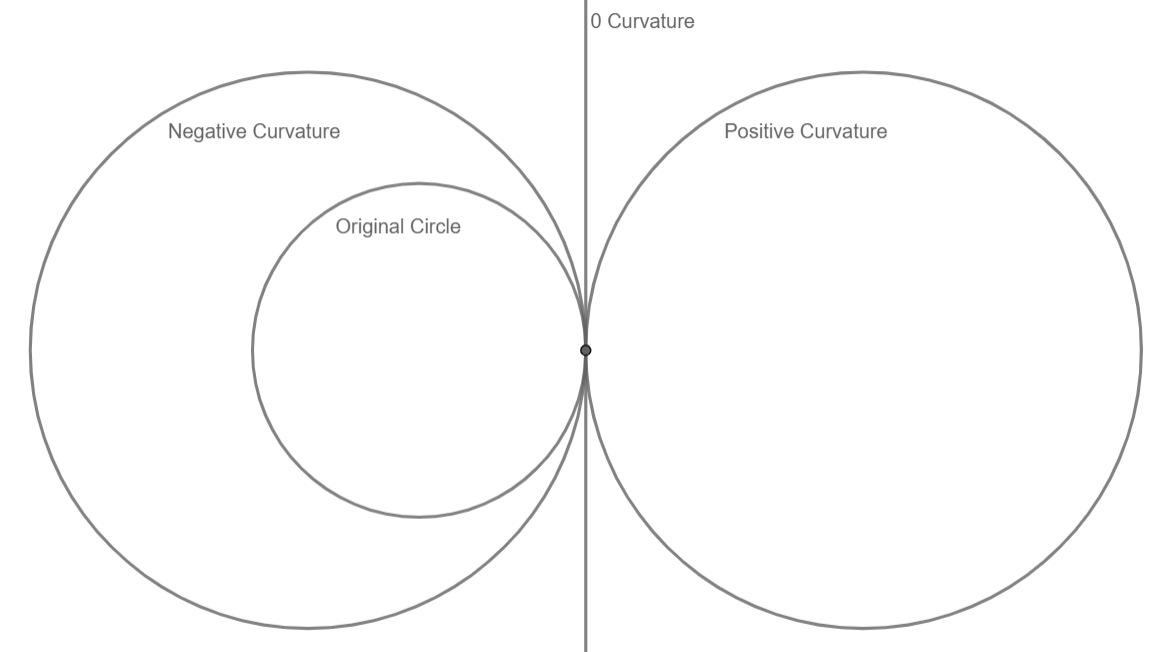
\includegraphics[width=.5\textwidth]{Figure 1 - Types of Curvatures.png}
\caption{Types of Curvatures with respect to the Original Circle.}
\end{figure}

We call a configuration of four pairwise tangent circles (with or without infinite radius) a \textbf{Descartes' Circle configuration}. Observe that we have exactly four Descartes' Circle configurations (check that it is impossible for one circle and three lines to be all mutually tangent to one another). See figure 2. 

\begin{figure}[ht]
\centering
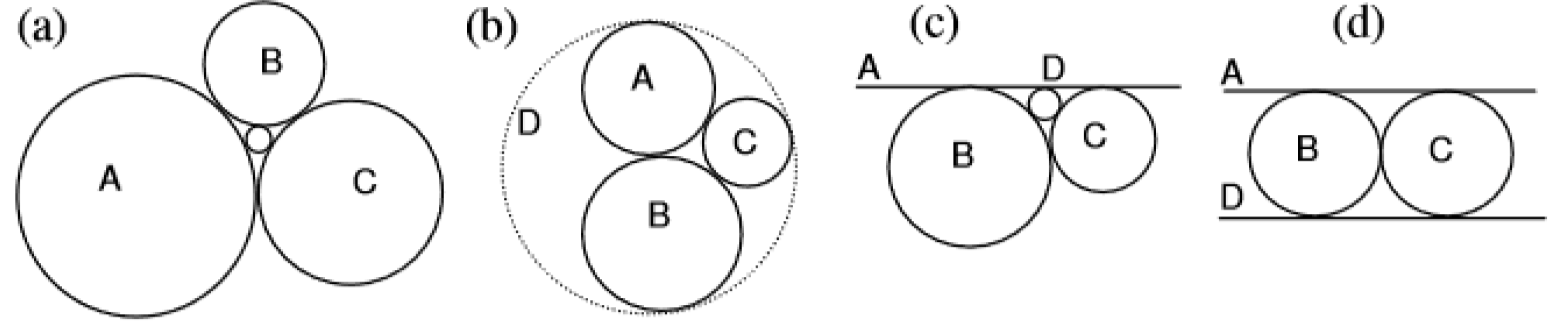
\includegraphics[width=.5\textwidth]{Figure 2 - Descartes' Circle Configs Bigger Still.png}
\caption{The four Descartes' Circle configurations.}
\end{figure}

Now we are ready to state the main theorem.

\subsection{The Moment We've Been Waiting For}
\textbf{Descartes' Circle Theorem} states that, given a configuration of four mutually tangent circles, $\omega_1,\omega_2,\omega_3,\omega_4$, their curvatures, $c_1,c_2,c_3,c_4$, satisfy the follow relation: $$(c_1+c_2+c_3+c_4)^2=2(c_1^2+c_2^2+c_3^2+c_4^2).$$

This relation holds for all four configurations presented in figure 2. Cases (a) and (b) are standard. In case (c), we let $c_3=0$, and in case (d), we let $c_2=c_3=0$. For a proof of this theorem, see \href{https://brilliant.org/wiki/descartes-theorem/}{Brilliant's Trigonometry Proof.}

Descartes' Circle Theorem does not apply to four circles (with or without infinite radius) that are tangent at one and only one point. Such a set of circles are said to be coaxial. See figure 1 for an example of four coaxial circles.

Many times, we are given the radii/curvature of three of the circles and are asked to find the radius/curvature of the fourth. In such instances, we can isolate $c_4$ to get the equation $$c_4=c_1+c_2+c_3\pm 2\sqrt{c_1c_2+c_2c_3+c_3c_1}.$$ Of note is the fact that there are actually two solutions for $c_4$ as indicated by the $\pm$ sign. This is due to the fact that there are always two such circles that are tangent to the other three in a Descartes' Circle configuration. 

Note that we could also write Descartes' Circle Theorem using summations as $$\left(\sum_{j=1}^4 c_j\right)^2=2\left(\sum_{j=1}^4 c_j^2\right)$$ or using a matrix as $$\begin{bmatrix} c_1&c_2&c_3&c_4\end{bmatrix} \begin{bmatrix}-1&1&1&1\\1&-1&1&1\\1&1&-1&1\\1&1&1&-1 \end{bmatrix}  \begin{bmatrix} c_1\\c_2\\c_3\\c_4\end{bmatrix}=0.$$ However, it is probably simplest to use the simplified form.
\subsection{Complex Descartes' Circle Theorem}
We can actually get some information about the centers of the circles in a Descartes' Circle configuration as well. In the complex plane, if we let the centers of circles $\omega_j$ be the complex number $z_j=x_j+iy_j$ for $j=1,2,3,4$, then $$\left(\sum_{j=1}^4 c_jz_j\right)^2=2\left(\sum_{j=1}^4 (c_jz_j)^2\right)$$ where $c_j$ is the curvature of circle $\omega_j$. 

Once $c_4$, the curvature of $\omega_4$, has been found using the original Descartes' Circle Theorem, we can find $z_4$, the center of $\omega_4$, with the following formula: $$z_4=\frac{c_1z_1+c_2z_2+c_3z_3\pm 2\sqrt{c_1z_1c_2z_2+c_2c_3z_2z_3+c_3c_1z_3z_1}}{c_4}.$$ Note that there are two solutions for $z_4$ which correspond to the two solutions for $c_4$. However, the $\pm$ sign in the formula for $k_4$ does not necessarily correspond to the $\pm$ sign in the formula for $z_4$: be careful here!
\section{The Soddy-Gosset Theorem}
Descartes' Circle Theorem actually generalizes to $n$ dimensions. 

\textbf{The Soddy-Gossett Theorem} states that, in a $n$-dimensional Euclidean space, given a configuration of $n+2$ mutually tangent spheres, $\omega_1,\omega_2,\omega_3,...,\omega_n$, their curvatures, $c_1,c_2,c_3,...,c_n$, satisfy the follow relation: $$\left(\sum_{j=1}^{n+2} c_j\right)^2=n\left(\sum_{j=1}^{n+2} c_j^2\right).$$ If $n=2$, this is just Descartes' Circle Theorem. This theorem is very non-trivial to prove and it requires a lot of advanced math. If you are curious, a proof can be found here on \href{https://math.stackexchange.com/questions/881777/proof-of-descartes-theorem}{Math Stack Exchange.}



Of course, in competition math, we mostly care about the $n=2$ case, but we will sometimes make use of the $n=3$ case as well. In these situations, we treat planes as spheres with infinite radius and thus curvature $0$. 
\section{Examples}
Now that we are sufficiently armed, let's kill some monsters! Err...solve some problems! Note that clicking the problem's source will take you to the corresponding AoPS thread where you can view the answers and solutions. If there are none, please post one (or tell me to post one). 

\subsection{Example 1. \href{https://artofproblemsolving.com/community/c4h2422437}{(2004 UQ/QAMT PS Competition 11-12 Problem 2)}}
\subsubsection{Problem.}
Three spherical melons, radius $9$ cm each, are placed on a flat table, each touching both the others. What is the radius of the largest orange that will sit on the table in the space between the $3$ melons? 
\subsubsection{Solution}
This is just an direct application of the Soddy-Gosset Theorem with $n=3$. Indeed, after treating the table as a sphere with curvature $0$, we have $$\left(0+\frac19+\frac19+\frac19+c_5  \right)=3\left(0^2+\frac{1}{9^2}+\frac{1}{9^2}+\frac{1}{9^2}+c_5^2 \right).$$ Simplifying and solving, we find that $c_5=\frac13$ so the radius or the orange is $3$ cm. 
\subsection{Example 2. \href{https://artofproblemsolving.com/community/c149h477544}{(Purple Comet 2012 HS Problem 22)}}
\subsubsection{Problem.}
The diagram below shows circles radius $1$ and $2$ externally tangent to each other and internally tangent to a circle radius $3$. There are relatively prime positive integers $m$ and $n$ so that a circle radius $\frac{m}{n}$ is internally tangent to the circle radius $3$ and externally tangent to the other two circles as shown. Find $m+n$.

\begincentering
\begin{asy}
import graph; size(5cm); 
real labelscalefactor = 0.5; 
pen dps = linewidth(0.7) + fontsize(10); defaultpen(dps); 
pen dotstyle = black;
draw(circle((8,2), 3)); 
draw(circle((8,1), 2)); 
draw(circle((8,4), 1)); 
draw((8,-1)--(8,5)); 
draw(circle((9.72,3.28), 0.86)); 
label("$ 2 $",(7.56,1.38),SE*labelscalefactor); 
label("$ 1 $",(7.6,4.39),SE*labelscalefactor); 
\end{asy}
\endcentering
\subsubsection{Solution.}
Applying Descartes' Circle Theorem to circles with curvatures $\frac11,\frac12,-\frac13$ (remember that negative sign!), we obtain $$\left(\frac11+\frac12-\frac13+c_4\right)^2=2\left(\frac{1}{1^2}+\frac{1}{2^2}+\frac{1}{(-3)^2}+c_4^2 \right).$$ Solving, we get \begin{align*} \left(\frac{7}6+c_4\right)^2&=2\left(\frac{49}{36}+c_4^2\right)\\ \frac{49}{36}+\frac{7}3 c_4+c_4^2&=\frac{49}{18}+2c_4^2\\ \frac{49}{36}+\frac{84}{36}c_4&=\frac{98}{36}+c_4^2\\ 36c_4^2-84c_4-49&=0 \end{align*} and the quadratic formula gives $$c_4=\frac{-(-84)\pm \sqrt{(-84)^2-4\cdot 36\cdot 49}}{2\cdot 36}=\frac{84\pm 0}{72}=\frac76.$$ Thus, the radius is $\frac76$ and the answer is $7+6=13$. 

Note that we only got back one solution since the two possible circles are congruent! If we were using Complex Descartes' Circle Theorem, however, we would get two different centers even though the radii/curvatures are the same.

To check our work, we can use $$c_4=c_1+c_2+c_3\pm 2\sqrt{c_1c_2+c_2c_3+c_3c_1}=\frac11+\frac12-\frac13+2\sqrt{\frac11\cdot\frac12-\frac12\cdot-\frac13-\frac13\cdot\frac11}=\frac76$$ which is what we got before. 

\subsection{Example 3. \href{https://artofproblemsolving.com/community/c4h71749p416082}{(2004 AMC 12A Problem 19)}}
\subsubsection{Problem.}
Circles $A,B,$ and $C$ are externally tangent to each other, and internally tangent to circle $D$. Circles $B$ and $C$ are congruent. Circle $A$ has radius $1$ and passes through the center of $D$. What is the radius of circle $B$?
\subsubsection{Solution.}
From the given information, we see that the signed radius of circle $D$ is $-2$ so its curvature is $-\frac12$. The curvature of circle $A$ is clearly $\frac11$. Let the curvature of circle $B$ and circle $C$ be $c$. Applying Descartes' Circle Theorem, we obtain $$\left(\frac11+c+c-\frac12\right)^2=2\left(\frac{1}{1^2}+c^2+c^2+\frac{1}{-(2)^2}\right).$$  Solving for $c$, we have \begin{align*} \left(\frac12+2c\right)^2&=2\left(\frac54+2c^2\right)\\ \frac14+2c+4c^2&=\frac52+4c^2\\ 2c&=\frac94\\ c&=\frac98 \end{align*} so the radius of circle $B$ is $\frac89$. 

\subsection{Example 4. \href{https://artofproblemsolving.com/community/c4h64305p382541}{(2001 AMC 12 Problem 18)}}
\subsubsection{Problem.}
A circle centered at $A$ with a radius of $1$ and a circle centered at $B$ with a radius of $4$ are externally tangent. A third circle is tangent the first two and to one of their common external tangents as shown. The radius of the third circle is? 

\begin{asy}
size(250);
real r1 = 1;
real r2 = 3;
real r = (r1*r2)/((sqrt(r1)+sqrt(r2))**2);
pair A=(0,r1), B=(2*sqrt(r1*r2),r2);
dot(A); dot(B);
draw( circle(A,r1) );
draw( circle(B,r2) );
draw( (-1.5,0)--(7.5,0) );
draw( A -- (A+dir(210)*r1) );
label("$1$", A -- (A+dir(210)*r1), N );
draw( B -- (B+r2*dir(330)) );
label("$4$", B -- (B+r2*dir(330)), N );
label("$A$",A,dir(330));
label("$B$",B, dir(140));

draw( circle( (2*sqrt(r1*r),r), r ));
\end{asy}
\subsubsection{Solution.}
The common external tangent is a circle with curvature $0$. If we let the curvature of the third circle be $c_3$, we have $$\left(\frac11+\frac14+c_3+0\right)^2=2\left(\frac{1}{1^2}+\frac{1}{4^2}+c_3^2+0^2\right)$$ by Descartes' Circle Theorem. Solving, we get \begin{align*}\left(\frac54+c_3^2\right)&=2\left(\frac{17}{16}+c_3^2\right)\\ \frac{25}{16}+\frac52 c_3+c_3^2&=\frac{34}{16}+2c_3^2\\ 16c_3^2-40c_3+9&=0 \end{align*} and the quadratic formula tells us that $c_3=\frac94$. Hence, the radius of the third circle is $\frac49$.

\section{Problems}

The first ten problems should be quite approachable. Everything after that can be quite challenging - try them at your own risk.

\subsection{Problem 1. \href{https://artofproblemsolving.com/community/c6h2422942}{(2014 Saint Petersburg State University School Olympiad Finals, Grades 10-11 p6 v1)}}

In a spherical shell of radius $5$ are placed three metallic balls, two of which have radii $1$ and $4$. Find the maximum possible radius of the third ball.

\subsection{Problem 2. \href{https://artofproblemsolving.com/community/c4h2422452}{(2002 UQ/QAMT PS Competition 11-12 Problem 5)}}

You have a semicircle with diameter $AB$ of length $8$ cm, inside which are drawn non-overlapping semicircles of diameters $6$ cm and $2$ cm. A circle $C$ is drawn, touching all three semicircles as shown. Show that the perpendicular distance from the centre of this circle $C$ to the diameter $AB$ is equal to the diameter of the circle $C$.

\subsection{Problem 3. \href{https://artofproblemsolving.com/community/c4h2384801}{(2018 Belgium OMB Juniors p2)}}

A tunnel, the cross section of which is shown opposite, has two traffic lanes represented by half-discs of the same radius and a gas discharge duct represented by a smaller disc. The two half-discs and the small disc are tangent in pairs and tangent internally to a large disc of diameter equal to $12$ m. What is the diameter of the gas discharge pipe?

\begin{figure}[ht]
\centering
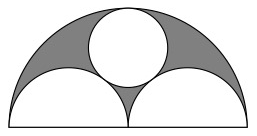
\includegraphics[width=.5\textwidth]{6.3.png}
\caption{Diagram for 6.3.}
\end{figure}



\subsection{Problem 4. \href{https://artofproblemsolving.com/community/c5h1379993}{(2017 AMC 12A Problem 16)}}

In the figure below, semicircles with centers at $A$ and $B$ and with radii $2$ and $1$, respectively, are drawn in the interior of, and sharing bases with, a semicircle with diameter $\overline{JK}$. The two smaller semicircles are externally tangent to each other and internally tangent to the largest semicircle. A circle centered at $P$ is drawn externally tangent to the two smaller semicircles and internally tangent to the largest semicircle. What is the radius of the circle centered at $P$?

\begin{figure}[ht]
\centering
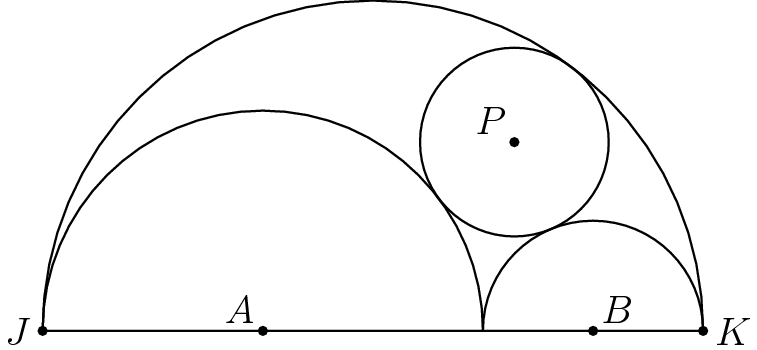
\includegraphics[width=.5\textwidth]{6.4.png}
\caption{Diagram for 6.4.}
\end{figure}


\subsection{Problem 5. \href{https://artofproblemsolving.com/community/c4h1515721}{(Reworded from AoPS)}}

Given three externally tangent circles of radii $3,4,5$, find the sum of the radii of the two circles which are respectively internally and externally tangent to the three original ones.

\subsection{Problem 6. \href{https://artofproblemsolving.com/community/c4h396448}{(From AoPS)}}

Two circles of radius 4 and 5 are tangent to each other and the common external tangent $\ell$. Between the two circles and the line is another circle that is tangent to both circles and the line. Find the radius of this circle.

\subsection{Problem 7. \href{https://artofproblemsolving.com/community/c4h2562133}{(2015 All-Siberian Qualifying 11.4)}}

In a semicircle with a radius of $18$ cm, a semicircle of radius $9$ cm is built on one of the halves of the diameter, and a circle is inscribed, touching the larger semicircle from the inside, the smaller semicircle from the outside and and the second half of the diameter. Find the radius of this circle.

\subsection{Problem 8. \href{https://artofproblemsolving.com/community/c4h2551282}{(2017 Izumrud Olympiad 10 v2 p2)}}

On segment $AC=12$, point $B$ is marked such that $AB = 4$. Using segments $AB$ and $AC$ as diameters, semicircles are constructed in the same half-plane with respect to the segment $AC$. Calculate the radius of the circle tangent to the constructed semicircles and $AC$.

\subsection{Problem 9. \href{https://artofproblemsolving.com/community/c4h2549180}{(2009 All-Siberian Correspondence 11.2)}}

Three identical balls of radius $1$ are located on the plane, each of which touches the other two and the plane. Find the radius of the fourth ball touching each of these three and the plane.

\subsection{Problem 10. \href{https://artofproblemsolving.com/community/c4h2562126}{(2015 All-Siberian Qualifying 9.3)}}

Inside a semicircle of radius $12$, there is a circle of radius $6$, and a small semicircle, touching each other in pairs, like shown in the figure. Find the radius of the small semicircle.

\begin{figure}[ht]
\centering
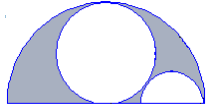
\includegraphics[width=.5\textwidth]{6.10.png}
\caption{Diagram for 6.10.}
\end{figure}

\subsection{Problem 11. \href{https://artofproblemsolving.com/community/c6h1541216p9332650}{(From AoPS)}}

There are four circle whose radii are $a,b,c,d$ such that $a\leq{b}\leq{c}\leq{d}$ and such that they are mutually externally tangent. Find the maximum value of $\frac{a}{d}$.

\subsection{Problem 12. \href{https://artofproblemsolving.com/community/c487h560347}{(2013-2014 Fall OMO #30)}}

Let $P(t) = t^3+27t^2+199t+432$.  Suppose $a$, $b$, $c$, and $x$ are distinct positive reals such that $P(-a)=P(-b)=P(-c)=0$, and \[
\sqrt{\frac{a+b+c}{x}} = \sqrt{\frac{b+c+x}{a}} + \sqrt{\frac{c+a+x}{b}} + \sqrt{\frac{a+b+x}{c}}. \] If $x=\frac{m}{n}$ for relatively prime positive integers $m$ and $n$, compute $m+n$.

\subsection{Problem 13. \href{https://artofproblemsolving.com/community/c5h623878}{(2015 AMC 12A #25)}}

A collection of circles in the upper half-plane, all tangent to the $x$-axis, is constructed in layers as follows.  Layer $L_0$ consists of two circles of radii $70^2$ and $73^2$ that are externally tangent.  For $k\geq 1$, the circles in $\textstyle\bigcup_{j=0}^{k-1} L_j$ are ordered according to their points of tangency with the $x$-axis.  For every pair of consecutive circles in this order, a new circle is constructed externally tangent to each of the two circles in the pair.  Layer $L_k$ consists of the $2^{k-1}$ circles constructed in this way.  Let $S=\textstyle\bigcup_{j=0}^6 L_j$, and for every circle $C$ denote by $r(C)$ its radius.  What is \[\sum_{C\in S}\dfrac1{\sqrt{r(C)}}?\]

\begin{figure}[ht]
\centering
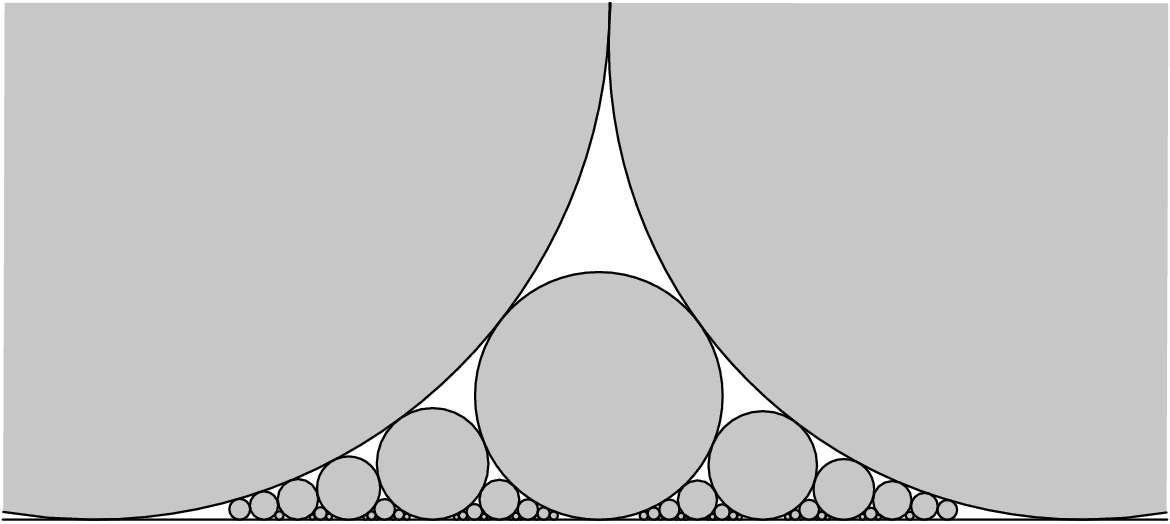
\includegraphics[width=.5\textwidth]{6.13.png}
\caption{Diagram for 6.13.}
\end{figure}


\subsection{Problem 14. \href{https://artofproblemsolving.com/community/c4h2423952}{(2008 UQ/QAMT PS Competition 11-12 p4)}}

$C_0$ is a circle of radius $10$ metres tangent to the ground. $C_1$ is a circle of radius $1$ millimetre, external to $C_0$ and tangent to both $C_0$ and the ground. For $n > 2, C_n$ is a circle tangent to $C_0, C_{n-1}$ and the ground. The diagram to the right shows the first few circles in this pattern (not to scale).
How many circles can be placed in this way (before they get too large to be tangential to $C_0$)?

\begin{figure}[ht]
\centering
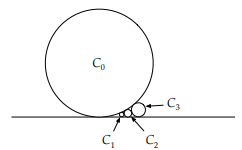
\includegraphics[width=.5\textwidth]{6.14.png}
\caption{Diagram for 6.14.}
\end{figure}

\section{Parting Words}

Thank you for reading this handout! I hope it explained Descartes' Circle Theorem well and was enjoyable to read. If you are interested in this topic, I would suggest looking into the Apollonian Gasket, the Shoemaker Knife, Arbelos Packings, Archemedian Circles, Farley/Ford Circles, and the optimal way to stack spheres. Also of interest should be Inversive Geometry which let's one destroy many of the aobve-mentioned problems. To get you started, \href{https://www.maa.org/sites/default/files/pdf/ebooks/pdf/EGMO_chapter8.pdf}{this book chapter} and \href{https://www.youtube.com/watch?v=CROeIGfr3gs}{this video} are both extremely good. 





\end{document}
